\documentclass[11pt]{article}
\usepackage[a4paper,margin=1.05in]{geometry}
\usepackage{amsmath,amssymb}
\usepackage{graphicx}
\usepackage{booktabs}
\usepackage{microtype}
\usepackage{xcolor}
\usepackage[colorlinks=true,linkcolor=blue!50!black,citecolor=blue!50!black,urlcolor=blue!60!black]{hyperref}

\newcommand{\F}{\mathbb{F}}
\newcommand{\dem}{\textsc{dem}}
\setlength{\parskip}{2pt}

\title{Circuit-level equivariance is code-dependent: obstruction in the
surface code, exactness in the honeycomb Floquet code, and consequences for
neural decoders}
\author{Daniel Olliver\\
\small Independent researcher, Auckland, New Zealand\\
\small \texttt{dwatces@gmail.com} \,\;
\href{https://github.com/dwatces/equivariant-quantum-ml}{\small github.com/dwatces/equivariant-quantum-ml}}
\date{June 2026}

\begin{document}
\maketitle

\begin{abstract}
\noindent
Symmetry-equivariant neural decoders for quantum error correction were
introduced by Egorov, Bondesan and Welling for the toric code at code
capacity, where the optimal decoder's symmetry group --- including
syndrome-dependent corrections to the logical labels --- can be derived
analytically from lattice paths. Real decoders, however, operate at circuit
level, on the detector error model (DEM) generated by a syndrome-extraction
circuit. We show that whether exact equivariance survives the passage to
circuit level is a property of the \emph{code}. For the surface code it does
not: an exhaustive search over 999 affine spacetime detector maps and a
constructive co-design search over 1{,}728 extraction schedules find no
exact twisted symmetry of the circuit-level DEM within the geometric
family, and we identify the
mechanism --- a mirror-axis ancilla would need a CNOT order equal to its own
reflection, which no order can be. For the honeycomb Floquet code an exact
$p3$ space group --- the color-preserving translations and $C_3$ rotations
--- survives even naive ancilla-compiled extraction (the color-cycling
elements survive as exact spacetime screws in the time bulk): trivalence
makes every check weight-2, reducing
schedule freedom to one bit per edge (automatically covariant) and hook
errors to weight one. We solve the symmetry action on the logical
observables directly from the DEM as a triple $(P, A, X)$ --- detector
permutation, $GL(2,\F_2)$ action on the two logical qubits, and a
syndrome-dependent twist --- verify it against every DEM mechanism group,
and validate the solver by blind recovery of the known analytic action on
the toric code. The $C_3$ rotation mixes the logical qubits ($A$ of order
3), so the correct equivariant decoder is a four-class, jointly-equivariant
model. On the honeycomb circuit-level task, a matched-parameter
unconstrained network remains at the majority-class baseline through 64{,}000
training samples, while the exactly-tied model reaches $0.806 \pm 0.003$ at
256{,}000 samples --- the tied model at 1{,}000 samples outperforms the
unconstrained model at 256{,}000, a $\geq 256\times$ sample-efficiency
separation. A noise-rate sweep finds the tied advantage at every rate
tested and locates the strict switch in a noise window around the gated
rate. On the surface code under phenomenological noise, where exact
symmetry exists below circuit level, the group elements that \emph{move} the
logical representative (twisted elements) carry essentially all of the
benefit. Code choice, not architecture choice, determines whether exact
equivariance is available to machine-learned decoders where devices actually
operate.
\end{abstract}

\section{Introduction}

Machine-learned decoders are now competitive with, and in some regimes ahead
of, hand-crafted decoders for quantum error correction: AlphaQubit
\cite{Bausch24} set the accuracy state of the art on Sycamore surface-code
data, and learned decoders adapt to real noise that analytic decoders model
imperfectly. The binding constraint in that program is \emph{data}: syndrome
samples from real hardware are scarce and expensive, which makes inductive
bias --- how much of the decoding function is built in rather than learned
--- the central design question.

The natural inductive bias for a topological code is its lattice symmetry.
Egorov, Bondesan and Welling (``The END'') \cite{Egorov23} formalized this
for the toric code at code capacity: the optimal decoder is equivariant
under the code's automorphism group \emph{provided} the output
representation is twisted --- the logical-class label transforms by a
group-element-dependent permutation composed with a syndrome-dependent
correction, because a symmetry maps a logical representative to a homologous
representative that differs by stabilizers. Their equivariant architecture,
built on a ``twisted global average pooling,'' beat both MWPM and prior
neural decoders, and --- a result we will return to --- their ablation found
that \emph{untwisted} pooling fails to learn at all.

The END's analysis lives at code capacity: perfect syndrome measurements, no
extraction circuit, with the twist derived analytically from lattice paths.
Real decoders consume the output of a \emph{syndrome-extraction circuit},
and the object they actually decode is the circuit's detector error model
(DEM): the hypergraph of elementary error mechanisms, the detectors they
flip, and the logical observables they cross. Whether the lattice symmetry
survives in the DEM is not guaranteed by the symmetry of the code: the
extraction schedule --- the order in which entangling gates touch each
ancilla --- imprints itself on the noise through hook errors, and schedules
are discrete objects with no obligation to respect the lattice's point
group.

This paper asks: \textbf{for which codes does exact (twisted) equivariance
survive at circuit level --- and what does the answer do to learned
decoders?}

Our contributions:

\begin{enumerate}
\item \textbf{A DEM-native solver for twisted symmetry actions} (\S3).
Given any stim circuit and a candidate detector permutation, we solve for
the action on the logical observables --- a pair $(A, X)$ with
$A \in GL(k, \F_2)$ acting on the $k$ logical bits and $X$ a syndrome-linear
twist --- from the DEM alone, by per-detector-set multiset equations, and
verify the result against every mechanism group exactly. No analytic path
construction is needed, which is what makes the method applicable at circuit
level. Blind-searched over all 24 label permutations on The END's own
setting (toric code, code capacity), the solver uniquely recovers their
analytic action --- including the $90^\circ$ rotation's logical swap and the
weight-$L$ stabilizer-path twists (\S3.2).

\item \textbf{An obstruction result for the surface code} (\S4). At circuit
level, no exact twisted symmetry of the unrotated surface-code DEM exists in
the geometric family: 999 affine spacetime maps (reflections, rotation,
time-reversal, shifts) all fail verification, and a constructive search over
1{,}728 extraction-schedule assignments --- including mirror-paired and
time-reversed families designed specifically to restore symmetry --- yields
zero verified schedules. We identify the obstruction: an ancilla on the
mirror axis would need a CNOT order whose hook-error prefixes equal their
own mirror image, and no permutation equals its own nontrivial
conjugate-reversal. Schedule co-design, recently an active topic for
distance preservation \cite{Kishony26,Fujiu25}, cannot rescue exact
equivariance for this code.

\item \textbf{An exactness result for the honeycomb Floquet code} (\S5).
The Hastings--Haah honeycomb code \cite{HH21} compiled with \emph{naive,
uniform} ancilla extraction carries an exact $p3$ space group ---
color-preserving translations and $C_3$ face rotations --- as a symmetry of
its circuit-level DEM, verified by exact multiset equality over all 4{,}020
mechanism groups at $L = 6$; the color-cycling elements survive as exact
time-bulk spacetime screws (composed with sub-round shifts). The mechanism
is trivalence: weight-2 checks leave one bit of schedule freedom per edge,
which is automatically covariant, and bound hook errors to weight one. No
schedule engineering is involved.

\item \textbf{The logical action and its decoder consequence} (\S5.3).
Solving $(A, X)$ on the honeycomb torus: translations act with $A = I$
(homology preserved, twist only), while $C_3$ acts with
$A = \left[\begin{smallmatrix}1&1\\1&0\end{smallmatrix}\right]$ --- an
order-3 element of $GL(2,\F_2)$ that \emph{mixes the two logical qubits}. A
scalar-label equivariant decoder therefore cannot express the code's
rotation symmetry at all; the correct formulation is a four-class (joint
two-bit) twisted-equivariant model,
$f(x)[c] = \tfrac{1}{|G|}\sum_g \mathrm{net}(\tilde x_g)[A_g c \oplus
X_g\!\cdot\!\tilde x_g]$. En route we find that the deterministic logical
wraps of an X-basis-initialized honeycomb memory exist only at one
termination phase in three (final readout in the Y basis,
$S \equiv 1 \bmod 3$) --- an operational fingerprint of the code's
logical-type rotation \cite{HH21} that our observable-derivation procedure
discovers automatically.

\item \textbf{Learning experiments} (\S6). (i) Surface code,
phenomenological noise: at matched parameters the twisted-invariant decoder
dominates plain at every training-set size ($d{=}3$: $+4.2$\,pp at $n{=}250$,
$\approx\!4\times$ sample efficiency; $d{=}5$: Klein-four reaches at
$n{=}4{,}000$ what plain reaches at 64{,}000, $>\!16\times$), and an element
ablation shows the \emph{twisted} elements --- those that move the logical
representative --- carry essentially all the benefit, while the $\chi = 0$
mirror contributes almost nothing. (ii) Honeycomb code, circuit-level noise:
the unconstrained matched-parameter MLP never leaves the majority-class
baseline through 64{,}000 samples; the $p3$-tied model reaches 0.744 at
64{,}000 and 0.806 at 256{,}000, and the tied model at 1{,}000 samples
exceeds the unconstrained model at 256{,}000 ($\geq 256\times$). Exact
equivariance here is not an efficiency multiplier but a learnability switch
--- consistent with, and sharpening, The END's untwisted-pooling ablation;
a noise-rate sweep (\S6.2) bounds the strict switch to a window around the
gated rate while the tied advantage holds at every rate.
(iii) Composing a translation-equivariant CNN backbone with the twisted
averaging improves the scarce-data regime further ($+3$ to $+6$\,pp over the
tied MLP at $10^3$--$10^4$ samples) and isolates a structural fact:
convolutional weight sharing cannot absorb the label twist --- on the same
conv backbone, explicit averaging over the very translations the convolution
already ``has'' adds $+21$\,pp, because the twist is a cocycle on the
output, not a feature symmetry (\S6.4).
\end{enumerate}

We close with what this does and does not imply for practical decoding
(\S7). Throughout, ``exact'' means exact multiset equality of DEM mechanism
groups under the candidate action --- a verification standard, not an
approximation.

\begin{figure}[t]
\centering
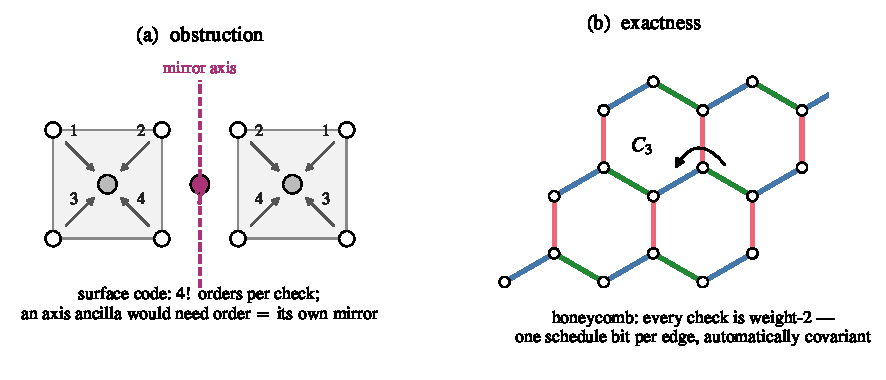
\includegraphics[width=0.96\linewidth]{figures/fig1_dichotomy.pdf}
\caption{\textbf{Why circuit-level equivariance is code-dependent.}
(a)~Surface code: each weight-4 check admits $4!$ CNOT orders; hook-error
prefixes depend on the order, and an ancilla on a mirror axis would need an
order equal to its own reflection, which no order is (\S4). (b)~Honeycomb
Floquet code: trivalence makes every check weight-2, leaving one schedule
bit per edge; a uniform sublattice rule is automatically covariant, so an
exact $p3$ space group survives in the circuit-level DEM under naive
extraction (\S5).}
\label{fig:dichotomy}
\end{figure}

\section{Background}

\subsection{Detector error models and decoding as classification}

A stabilizer memory experiment compiles to a Clifford circuit with noise; a
\emph{detector} is a parity of measurement records that is deterministic in
the noiseless circuit, and a \emph{logical observable} is such a parity that
reads out encoded information. The detector error model extracted from the
circuit (we use stim \cite{Gidney21}) is a list of elementary mechanisms
$(D_i, o_i, p_i)$: a set of flipped detectors, a mask of flipped
observables, and a probability. Decoding is the classification problem
syndrome $\to$ observable mask; MWPM \cite{Dennis02,Higgott23} is the
standard baseline; learned decoders \cite{Bausch24} fit the map from
samples.

\subsection{Twisted equivariance (after The END)}

A spatial symmetry $g$ of the code permutes detectors by some $P_g$. It does
not in general fix the chosen logical representatives; it maps them to
homologous representatives differing by stabilizer products, whose measured
values telescope into detector sums. The label therefore transforms as
$o \to A_g\, o \oplus X_g\!\cdot\!(P_g s)$ with $A_g$ a permutation-like
linear action on the logical bits and $X_g$ a fixed $\F_2$ matrix applied to
the permuted syndrome $s$. At code capacity on the toric code, $(A, X)$ can
be written down from lattice paths \cite{Egorov23}. The decoder respecting
this symmetry is the group-averaged, twist-corrected model used throughout
this paper.

\subsection{Codes and circuits}

\emph{Surface code:} stim's unrotated planar memory (Z basis), distances
3--11, phenomenological noise for \S6.1 (measurement-flip + data
depolarization, $p = 0.008$) and full circuit-level noise for \S4.

\emph{Honeycomb Floquet code \cite{HH21}:} torus, $L \times M$ cells (72
data qubits at $L = 6$), faces 3-colored, sub-round $s$ measures
color-$(s \bmod 3)$ edges in Pauli basis $(X,Y,Z)[s \bmod 3]$; detectors are
face inference windows compared across periods. We compile three extraction
modes --- direct two-body measurement (\texttt{mpp}), naive ancilla
extraction with a uniform ``A-sublattice-first'' gate order
(\texttt{cx-naive}), and an orbit-equivariant order (\texttt{cx-sym}) ---
and find (\S5) that the third is unnecessary: naive extraction is already
exactly symmetric. Circuit-level noise: single-qubit depolarization on data
each sub-round, two-qubit depolarization after each entangling gate, ancilla
preparation/readout flips, $p = 0.002$ for the decoding experiments (chosen
so the MWPM baseline operates in a learnable band; the noise-rate gate is
described in \S6.2).

\section{Solving twisted symmetry actions from the DEM}

\subsection{The per-group multiset method}

Group the DEM by detector set: $\mathrm{by\_v}[D]$ = multiset of $(o, p)$
over mechanisms with detector set $D$. A candidate action $(P, A, X)$ is an
exact symmetry iff for every $D$, the multiset
$\{(A o \oplus X\!\cdot\!\mathbf{1}_{P(D)},\, p)\}$ equals
$\mathrm{by\_v}[P(D)]$. Because $X$ enters only through the bit
$b(D) = X\!\cdot\!\mathbf{1}_{P(D)}$, each detector-set group yields a small
consistency problem: which label-offsets $b$ make the multisets match.
Groups with a unique consistent $b$ contribute linear equations
$X\!\cdot\!\mathbf{1}_{P(D)} = b$; groups consistent with several $b$'s are
unconstrained; any group with none rejects $(P, A)$. Gaussian elimination
over $\F_2$ solves the resulting system row-wise; a final pass re-verifies
every group against the solved action. Two practical notes: (i)~stim merges
mechanisms with identical detector sets, which is why the equations must be
extracted per \emph{group multiset} rather than per mechanism --- naive
mechanism-pairing generates false equations from probability collisions at
$d \geq 5$; (ii)~$X$ is unique only modulo directions invisible to every
mechanism set, so equivariance is exact on realizable syndromes (all
train/test data), which is the relevant statement for decoding.

\subsection{Validation: blind recovery of the analytic toric action}

On The END's setting --- toric code, code capacity, i.i.d.\ depolarizing ---
we ran the solver with \emph{no analytic input}, searching all 24
permutations of the four logical labels for each generator. For every
element the verifying $A$ is unique and matches the analytic action
\cite{Egorov23}: translations and the mirror fix the labels ($A = I$) with
twist $\chi$ supported on a weight-$L$ stabilizer path along the moved
representative; the $90^\circ$ rotation swaps
$\bar X_1 \leftrightarrow \bar X_2$ and $\bar Z_1 \leftrightarrow \bar Z_2$
with a single weight-$L$ path twist. (Run time: ${\sim}1$\,s; Appendix~D.)
This validates the solver in the one setting with a known analytic answer,
and licenses its use at circuit level, where none exists.

\begin{figure}[t]
\centering
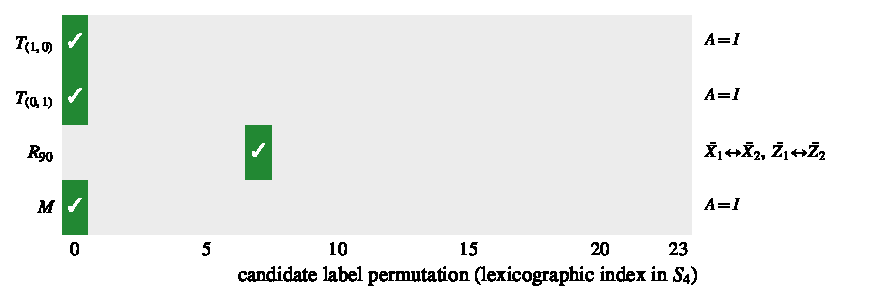
\includegraphics[width=0.96\linewidth]{figures/fig2_toric_bridge.pdf}
\caption{\textbf{Blind validation on The END's setting} (toric code, code
capacity, $L = 6$). For each lattice generator the $(A, X)$ solver is run
against all 24 candidate label permutations; exactly one verifies (green),
and it matches the analytic action of \cite{Egorov23}, including the
$90^\circ$-rotation logical swap. Data:
\texttt{runs/toric\_end\_bridge.json}.}
\label{fig:bridge}
\end{figure}

\section{Surface code: circuit-level obstruction}

\textbf{Affine family (999 maps).} At circuit level (full extraction
circuits, stim-generated, $d = 3$ and $5$) we tested every affine spacetime
candidate $P(x, y, t) = (\sigma(x, y), \pm t + \Delta t)$ with
$\sigma \in \{\mathrm{mirror}_x, \mathrm{mirror}_y, C_2,
\mathrm{identity}\}$, time reversal, and shifts $\Delta \in [-2, 2]^3$:
\textbf{zero} candidates verify, at either distance. This family is
exhaustive for the geometric question: any DEM symmetry implementing a
spacetime isometry of the memory experiment must act on detector
coordinates as exactly such an affine map (point-group element composed
with shifts and possibly time reversal), so what lies outside the family is
by construction the non-geometric automorphism sector, which carries no
spatial weight-sharing interpretation and is scoped out below. The
extraction schedule's hook errors de-symmetrize the DEM: a hook error is a
weight-2 data error created mid-extraction whose support depends on the
CNOT order, and the orders do not transform into each other under the
lattice maps.

\textbf{Schedule co-design (1{,}728 schedules).} Could the schedule be
\emph{chosen} to restore symmetry? We searched three families at $d = 3$
(rounds $=$ 3, full circuit noise) with hard gates: G1 no gate collisions,
G2 deterministic detectors, G3 circuit distance preserved, G4 exact
twisted-symmetry verification. Family A (uniform per-orientation orders,
576): 96 collision-free, 16 pass G1--G3, \textbf{0 pass G4}. Family B
(mirror-paired halves, 576): all 576 collide --- the center-column
ancilla's step-$k$ east target is exactly the mirrored neighbor's step-$k$
west target. Family C (mirror-paired with time-reversed right half, 576):
the collision is fixed by construction, 32 valid, 8 pass G1--G3, \textbf{0
pass G4}.

\textbf{The obstruction.} An ancilla lying \emph{on} the mirror axis must
have a CNOT order whose hook-error prefix sets are invariant under the
mirror's east--west exchange; concretely the order would have to equal its
own nontrivial reversal-conjugate, which no permutation does. This is why
both engineered families fail at the axis. The recent schedule-design
literature optimizes a different objective --- keeping hook errors off the
logical operators to preserve circuit distance \cite{Kishony26,Fujiu25} ---
and succeeds at it; exact DEM equivariance is a strictly stronger demand,
and for this code it is unachievable within the geometric family.
(Non-geometric DEM automorphisms found by graph tools \cite{Koutsioumpas25}
remain possible; they lack the spatial weight-sharing interpretation that
motivates equivariant architectures, and we leave them open.)

\section{Honeycomb Floquet code: circuit-level exactness}

\subsection{Trivalence removes the schedule obstruction}

Because the honeycomb lattice is trivalent, every check is weight-2: each
extraction is two entangling gates, schedule freedom is a single bit per
edge (``which endpoint first''), and hook errors have weight $\leq 1$ on
data --- they merge into existing single-qubit mechanism classes instead of
creating orientation-dependent weight-2 classes. A uniform sublattice rule
(``A-endpoint first'') is automatically covariant under every
sublattice-preserving lattice map. The contrast with the surface code's $4!$
candidate orders per plaquette accounts for the obstruction--exactness
dichotomy of this paper.

\subsection{Verified symmetry of the circuit-level DEM}

With the schedule's period-3 color structure, the point group splits into
color-preserving elements (pure spatial symmetries of the scheduled
circuit), color-cycling elements (exact only when composed with a $\pm 1$
sub-round shift --- spacetime \emph{screws}), and color-transposing elements
(paired with time reversal; classified, untested). Verified at $L = 6$
($R = 9$, 276 detectors, $p = 0.008$) by full-DEM multiset equality:
translations $T(1,1)$, $T(2,2)$ and $C_3$ about a face are exact over the
full DEM (4{,}020 groups) in \emph{all three} extraction modes including
naive; the $C_3$-about-a-vertex screw is exact in the time bulk, with the
init transient pinned to absolute sub-round 7 excluded by a bulk margin (the
temporal analogue of a spatial boundary). The orbit-engineered schedule
equals the naive one everywhere --- we record this because the fact that
engineering is unnecessary is itself part of the result.

\subsection{Logical observables, the termination effect, and $GL(2,\F_2)$}

To decode we need observables. We \emph{derive} them rather than construct
them: sampling the noiseless circuit and taking the $\F_2$ null space of the
record matrix yields every deterministic record parity; quotienting by the
detector span leaves the trackable logicals. This procedure produced two
findings:

\emph{Termination.} With $|+\rangle^{\otimes n}$ initialization, the
deterministic wrap pair exists only when the memory is terminated one
sub-round after a complete period, with transversal readout in the Y basis
($S \equiv 1 \bmod 3$); X- and Z-basis terminations carry zero deterministic
wraps. This is the honeycomb code's logical-type rotation \cite{HH21}
appearing as an operational constraint, found empirically by sweeping the
termination phase. The surviving observables are ``moving logical''
spacetime tubes --- at $L = 6$, weights 116 and 128 records, of which only 8
and 14 are data records --- and the experiment must be terminated with the
right structural detectors (initialization-round checks, virtual-round
closures reconstructing the missing color from data pairs, and final
window-vs-data comparisons) for the memory to have no undetectable boundary
errors; the construction is gate-checked by noiseless determinism throughout
(Appendix~C).

\emph{The logical action.} Solving $(A, X)$ for the nine-element group
$p3_9 = \{C_3^a\, T(2,2)^b\}$ (a closed abelian subgroup of $p3$ at $L = 6$;
$C_3$ and $T(2,2)$ commute because $R(2,2) \equiv (2,2) \bmod 6$):

\begin{center}
\begin{tabular}{lll}
\toprule
element class & $A$ & twist \\
\midrule
$T_{22}$, $T_{44}$ & $I$ & $\chi$-weights up to 168 \\
$C_3$, $C_3 T$ &
$\left[\begin{smallmatrix}1&1\\1&0\end{smallmatrix}\right]$ (order 3) &
nonzero \\
$C_3^2$, $C_3^2 T$ &
$\left[\begin{smallmatrix}0&1\\1&1\end{smallmatrix}\right] =
\left[\begin{smallmatrix}1&1\\1&0\end{smallmatrix}\right]^2$ & nonzero \\
\bottomrule
\end{tabular}
\end{center}

\noindent verified against all 4{,}584 mechanism groups of the decoding
circuit ($p = 0.002$, naive extraction, observables included). None of this
is specific to $L = 6$: the construction gates reproduce the same action at
$L = 3$, and at $L = 9$ (810 detectors, 10{,}314 mechanism groups, $T(3,3)$
replacing $T(2,2)$ for closure) the termination effect reproduces (exactly
two deterministic wraps, again only at $S \equiv 1 \bmod 3$ with Y readout),
$C_3$ solves with the identical order-3 matrix, and the nine-element closure
verifies in full. Translations preserve the homology classes; \textbf{$C_3$
mixes the two logical qubits}, consistent with the automorphism picture of
Floquet codes \cite{Davydova24,Kobayashi23} --- here appearing not as a
logical gate to be exploited but as a constraint the decoder must respect. A
scalar-label equivariant decoder cannot express this symmetry; the correct
model is four-class and jointly equivariant,
\begin{equation}
f(x)[c] \;=\; \frac{1}{|G|} \sum_{g}
\mathrm{net}(\tilde x_g)\!\left[\, A_g\, c \,\oplus\, X_g \!\cdot\! \tilde
x_g \,\right], \qquad \tilde x_g = P_g^{-1}\text{-permuted } x,
\end{equation}
which is exactly invariant on realizable syndromes (measured deviation
$7.5 \times 10^{-9}$; the gauge caveat of \S3.1 is why the probe uses
sampled shots).

\section{Learning experiments}

Protocol common to all experiments: matched parameter counts across arms
(the tied models share one backbone evaluated $|G|$ times --- parameters are
matched, FLOPs are not, noted where relevant), Adam with learning rate
$10^{-3}$ and batch size 256, a fixed budget of 4{,}000 steps (20{,}000 for
the large-$n$ and scale arms), 5 random seeds (3 for the large-$n$
extension, 2 for the scale ablation; uncertainties are standard deviations
across seeds), 200{,}000-shot test sets, accuracy $=$ exact match of the
observable mask (joint over both logicals where two exist). Baselines: MWPM
via pymatching on the decomposed DEM, and the majority class. Total compute
is modest: all MLP experiments ran on one consumer GPU (GTX 1070), the CNN
sweeps on single A10G instances; the full experimental record behind this
paper is a few tens of GPU-hours. These are inductive-bias measurements at
matched parameters, not decoder benchmarks: we report accuracy at fixed
noise rates --- the evidence class of The END's code-capacity study
\cite{Egorov23} --- rather than per-round logical-error or threshold
curves, which would require competitive backbones (\S7); \S\ref{sec:switch}
includes a noise-rate robustness sweep.

\subsection{Surface code, phenomenological noise: twisted elements carry
the value}
\label{sec:surface}

$d = 3$ (memory-Z, $p = 0.008$, MWPM 0.9948; 5 seeds): the
$C_2$-twisted-invariant decoder beats plain at every $n$ ---
$0.9791 \pm .004$ vs $0.9371 \pm .007$ at $n = 250$ ($+4.2$\,pp), reaching
$0.9943 \pm .0002$ at 64{,}000 against MWPM 0.9948, where plain lags
(0.9908); the twisted model at 16{,}000 already exceeds plain at 64{,}000
(0.9921 vs 0.9908), $\approx 4\times$ sample efficiency.

$d = 5$ (MWPM 0.9994), element ablation at matched everything:

\begin{center}
\begin{tabular}{lcccc}
\toprule
$n$ & plain & mirror$_x$ ($\chi{=}0$) & $C_2$ (twisted) & Klein-4 \\
\midrule
250 & 0.8154 & 0.8151 & 0.8847 & \textbf{0.8942} \\
4{,}000 & 0.8483 & 0.8624 & 0.9253 & \textbf{0.9389} \\
64{,}000 & 0.9169 & 0.9295 & 0.9721 & \textbf{0.9797} \\
\bottomrule
\end{tabular}
\end{center}

Klein-4 at 4{,}000 exceeds plain at 64{,}000: $>16\times$. The mirror that
\emph{fixes} the logical representative ($\chi = 0$) contributes almost
nothing; the elements that move it carry the benefit. Our reading: the twist
supplies exactly the nonlocal label-consistency structure the decoder
otherwise has to infer from data --- the twist is not a nuisance but the
signal. At 1M samples and a $5\times$ longer step budget Klein-4 holds its
lead (0.9951 vs 0.9863) and closes to 0.4\,pp of MWPM. Capacity limits,
reported in full: the 2-layer MLP family saturates by $d = 7$ (plain falls
below majority; Klein-4 rescues $+15$\,pp but plateaus), fails entirely at
$d \geq 9$, and a 3D-CNN backbone moves the $d = 7$ ceiling to
${\approx}0.925$ at 16k samples with the same plateau thereafter. Correlated
pair-noise grows the symmetry advantage ($+11$\,pp at 64k) but does not let
any arm beat MWPM here; we claim no MWPM superiority anywhere in this paper.

\begin{figure}[t]
\centering
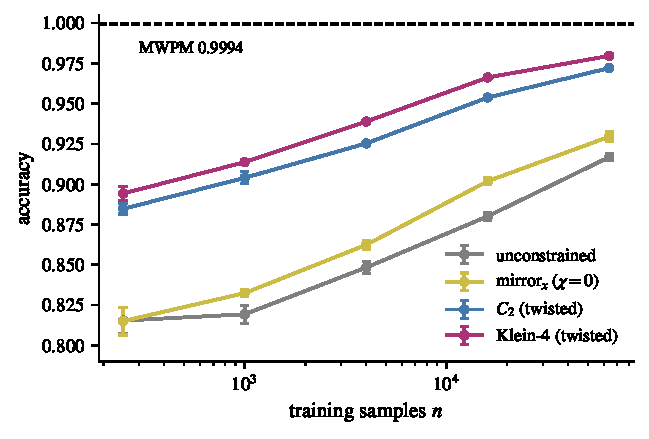
\includegraphics[width=0.62\linewidth]{figures/fig4_surface_elements.pdf}
\caption{\textbf{The twisted elements carry the benefit} (surface code
$d = 5$, phenomenological noise, matched parameters, 5 seeds). The
$\chi = 0$ mirror tracks the unconstrained baseline; the twisted $C_2$ and
Klein-4 arms dominate at every $n$ --- Klein-4 at 4{,}000 samples exceeds
unconstrained at 64{,}000 ($>16\times$). Data:
\texttt{runs/equiv\_decoder\_d5.json}, \texttt{\_d5b.json}.}
\label{fig:elements}
\end{figure}

\subsection{Honeycomb code, circuit-level noise: a learnability switch}
\label{sec:switch}

$L = 6$, $R = 9$, MY termination, naive extraction, $p = 0.002$ (noise
gate: $p$ chosen by halving from 0.008 until MWPM joint accuracy lands in a
learnable band; final MWPM 0.9471, majority 0.2908, flip rate 0.71 --- a
well-mixed four-class task). Matched 63{,}236-parameter MLP backbone:

\begin{center}
\begin{tabular}{lccc}
\toprule
$n$ & plain & $C_3$-tied (3 elements) & $p3_9$-tied (9 elements) \\
\midrule
250 & $0.2575 \pm .005$ & $0.2820 \pm .004$ & $\mathbf{0.3633 \pm .012}$ \\
1{,}000 & $0.2665 \pm .003$ & $0.3021 \pm .004$ & $\mathbf{0.4037 \pm .006}$ \\
4{,}000 & $0.2721 \pm .001$ & $0.3226 \pm .004$ & $\mathbf{0.4698 \pm .003}$ \\
16{,}000 & $0.2741 \pm .000$ & $0.3488 \pm .001$ & $\mathbf{0.6005 \pm .009}$ \\
64{,}000 & $0.2899 \pm .002$ & $0.5145 \pm .004$ & $\mathbf{0.7443 \pm .004}$ \\
\bottomrule
\end{tabular}
\end{center}

The unconstrained network never leaves the majority baseline. With $4\times$
more data and $5\times$ more steps it finally departs from it
($0.3907 \pm .001$ at $n = 256{,}000$) --- at which point the tied model is
at $0.8060 \pm .003$, and the tied model at $\mathbf{n = 1{,}000}$ (0.4037)
\textbf{still exceeds plain at} $\mathbf{n = 256{,}000}$: a $\geq 256\times$
sample-efficiency separation, against ${\approx}4\times$ ($d{=}3$) and
$>16\times$ ($d{=}5$) where the exact symmetry lives below circuit level. On
the code whose circuit-level DEM is exactly symmetric, equivariance is the
difference between not learning and learning --- the circuit-level
sharpening of The END's untwisted-pooling ablation.

To exclude a capacity artifact, we ran a pre-registered scale ablation
(predictions logged in the script before the run): at $7.1\times$ the
parameters ($h = 512$; 449{,}540) and $22.5\times$ ($h = 1024$; 1{,}423{,}364)
the unconstrained MLP still sits at the majority baseline at $n = 64{,}000$
($0.2858 \pm .001$ and $0.2862 \pm .001$ vs majority 0.2908), and at
$n = 256{,}000$ reaches only $0.3602 \pm .001$ --- no better than the narrow
model. Width does not help the tied model either: $p3_9$ at $h = 512$ gives
0.7386/0.8007 at 64k/256k versus 0.7443/0.8060 at $h = 128$. Together with
the convolutional backbone swap of \S6.4, this identifies the residual gap
to MWPM as a property of the architecture class, not of parameter count or
tying strategy.

\textbf{Noise-rate robustness.} A pre-registered sweep at
$p \in \{0.001, 0.002, 0.004\}$ (fresh 200k test sets per rate, 3 seeds)
bounds the switch claim in both directions:

\begin{center}
\begin{tabular}{lcccccc}
\toprule
$p$ & MWPM & majority & plain@4k & $p3_9$@4k & plain@64k & $p3_9$@64k \\
\midrule
0.001 & 0.9956 & 0.4086 & 0.3993 & \textbf{0.8544} & 0.6353 & \textbf{0.9625} \\
0.002 & 0.9471 & 0.2908 & 0.2717 & \textbf{0.4676} & 0.2890 & \textbf{0.7434} \\
0.004 & 0.6226 & 0.2536 & 0.2501 & 0.2544 & 0.2511 & 0.2615 \\
\bottomrule
\end{tabular}
\end{center}

The tied-over-plain ordering holds in every $(p, n)$ cell, MWPM is unbeaten
everywhere, and the solved $(A, X)$ action is bit-identical across rates, as
its structural origin requires. The registered prediction (strict switch at
every rate) is partially violated at both ends, and we report it as such:
at $p = 0.001$ the plain model escapes the baseline at 64{,}000 samples
($0.6353 \pm .001$) while remaining 33\,pp behind the tied model, whose
4{,}000-sample accuracy (0.8544) still exceeds plain at 64{,}000
($>16\times$); at $p = 0.004$ neither arm escapes baseline at these sample
sizes (tied $0.2615 \pm .001$ vs majority 0.2536, and MWPM itself falls to
0.62). The strict switch --- plain pinned at the majority baseline through
64{,}000 samples --- is a property of the gated rate; the sharper statement
the sweep supports is that exact tying \textbf{widens the noise window in
which the task is learnable at all} at fixed capacity and data.

Limitations: $p3_9$ at 256k remains 14.1\,pp below MWPM (architecture
class, not data or width --- the curve is unsaturated and $4\times$ width
does not move it); 20k-step training at fixed $n = 64$k mildly overfits
relative to 4k steps on the tied arms (0.7306 vs 0.7443); the scale arms use
2 seeds and the noise sweep 3, at $n \in \{4\text{k}, 64\text{k}\}$ only.

\begin{figure}[t]
\centering
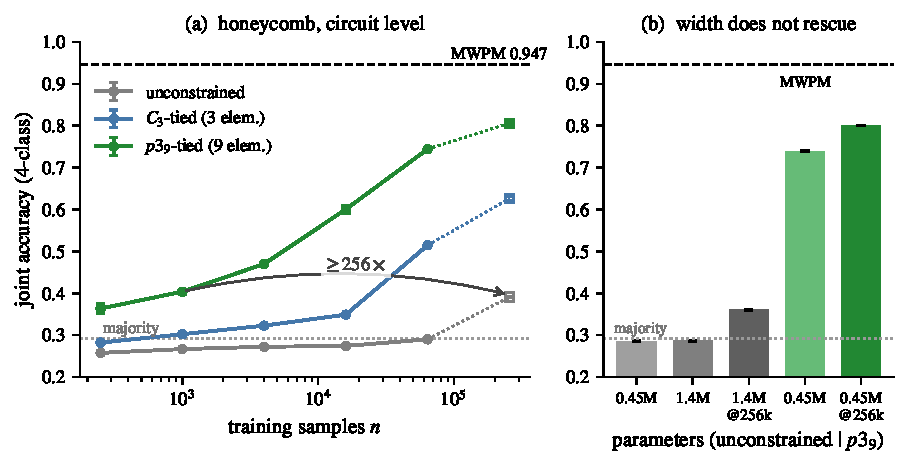
\includegraphics[width=0.96\linewidth]{figures/fig3_honeycomb_learning.pdf}
\caption{\textbf{Equivariance as a learnability switch} on the honeycomb
circuit-level task ($L = 6$, $p = 0.002$, MWPM 0.9471, majority 0.2908).
(a)~Matched 63k-parameter backbones, 5 seeds; open squares are the 256k
extension (3 seeds, 20k steps). The unconstrained MLP stays at the majority
baseline through 64{,}000 samples; the $p3_9$-tied model reaches 0.806 at
256{,}000, and at $n = 1{,}000$ already exceeds the unconstrained model at
$n = 256{,}000$ (arrow): $\geq 256\times$. (b)~Pre-registered scale
ablation: $7\times$--$22.5\times$ more parameters do not wake the
unconstrained model, and $4\times$ width does not move the tied model ---
the residual MWPM gap is architecture class, not capacity. Data:
\texttt{runs/honeycomb\_decoder\{,\_bign,\_scale\}.json}.}
\label{fig:switch}
\end{figure}

\subsection{What the comparison across codes says}

Identical backbones, identical training protocol, comparable detector
counts (240--588 vs 360): the surface-code architecture benefits from
symmetry below circuit level and \emph{cannot} be given exact symmetry at
circuit level (\S4); the honeycomb architecture is handed exact
circuit-level symmetry by the geometry and converts it into the largest
separations we measure. The lattice that buys nothing as a learned-model
\emph{input geometry} (our long-running negative results on hexagonal
inductive bias elsewhere) buys everything as the generator of the
\emph{code's} symmetry group.

\subsection{Composition with convolutional translation tying --- and what
weight sharing cannot do}
\label{sec:cnn}

We replace the MLP backbone with a 46{,}644-parameter 3D CNN over the
(time, face$_i$, face$_j$) detector grid --- circular padding on the torus
dimensions, so the convolution is natively translation-equivariant --- and
compose it with the same exact 4-class twisted averaging (invariance probe
$7.5 \times 10^{-9}$). Three questions (5 seeds, same protocol):

\begin{center}
\begin{tabular}{lcccc}
\toprule
$n$ & CNN (plain) & CNN + $C_3$ (3 el.) & CNN + $p3_9$ (9 el.) &
MLP + $p3_9$ (ref.) \\
\midrule
250 & $0.2555 \pm .005$ & $0.2810 \pm .009$ & $\mathbf{0.3647 \pm .011}$ & 0.3633 \\
1{,}000 & $0.2649 \pm .003$ & $0.3021 \pm .008$ & $\mathbf{0.4337 \pm .012}$ & 0.4037 \\
4{,}000 & $0.2732 \pm .002$ & $0.3393 \pm .006$ & $\mathbf{0.5291 \pm .008}$ & 0.4698 \\
16{,}000 & $0.2820 \pm .003$ & $0.4055 \pm .007$ & $\mathbf{0.6351 \pm .013}$ & 0.6005 \\
64{,}000 & $0.3184 \pm .007$ & $0.5380 \pm .008$ & $\mathbf{0.7502 \pm .015}$ & 0.7443 \\
\bottomrule
\end{tabular}
\end{center}

First, the translation prior alone does \emph{not} rescue learnability: the
unconstrained CNN sits at or near the majority baseline through 16{,}000
samples and reaches only 0.318 at 64{,}000. Second, the composition pays
where data is scarce: CNN+$p3_9$ exceeds MLP+$p3_9$ by $+3.0/+5.9/+3.5$\,pp
at $n = 1{,}000/4{,}000/16{,}000$, converging by 64{,}000 (0.750 vs 0.744);
the ${\approx}0.75$ ceiling at 64{,}000 --- some 20\,pp below MWPM --- is
unmoved by the backbone change, identifying the remaining gap as
architecture class rather than tying strategy (and not raw width ---
\S6.2's scale ablation), consistent with the surface-code $d = 7$ CNN
plateau (\S6.1). Third, on the \emph{same convolutional backbone}, going
from $C_3$-only averaging to the full nine-element group adds $+21$\,pp at
64{,}000 --- even though convolutions are already translation-equivariant.
The reason is that the label twist under translations ($A = I$ but
$\chi \neq 0$) is a cocycle on the \emph{output}, invisible to feature-level
weight sharing: convolution can share features across translated syndromes,
but only the twisted average makes the \emph{label} transform correctly.
Weight sharing handles the features; the twist must be handled explicitly.
Together with The END's pooling ablation and the element ablation of \S6.1,
this isolates a design rule for equivariant decoders: the syndrome-dependent
label correction is not an implementation detail of the symmetry --- it is
the component that carries the benefit.

\begin{figure}[t]
\centering
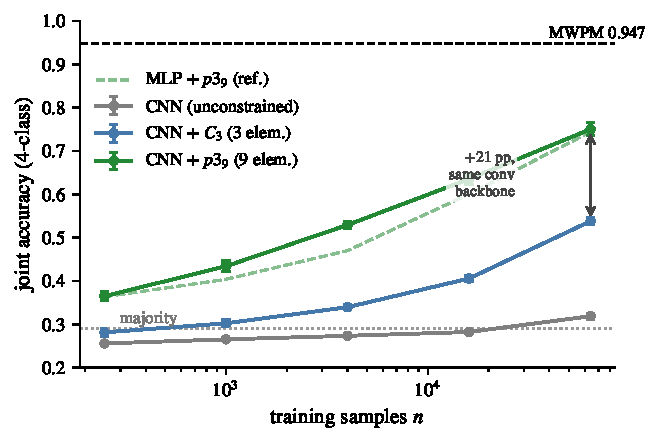
\includegraphics[width=0.62\linewidth]{figures/fig5_cnn_composition.pdf}
\caption{\textbf{Convolutional weight sharing cannot absorb the label
twist} (honeycomb task, 46{,}644-parameter 3D-CNN backbones, 5 seeds). The
translation-equivariant CNN alone stays near majority; composing it with
the exact twisted averaging pays $+3$--$6$\,pp over the tied MLP where data
is scarce; and on the same conv backbone the full nine-element group adds
$+21$\,pp at 64{,}000 over $C_3$-only averaging --- the twist is a cocycle
on the output, invisible to feature weight sharing. Data:
\texttt{runs/honeycomb\_decoder\_cnn.json}.}
\label{fig:cnn}
\end{figure}

\section{Discussion}

\textbf{What we claim.} (i) Exact twisted equivariance of the decoding
problem is a circuit-level property that depends on the code, decidable by
the DEM solver of \S3; (ii) for the surface code it is obstructed
structurally, not for want of schedule engineering; (iii) for the honeycomb
Floquet code it holds exactly with zero engineering, the logical action
includes a $GL(2,\F_2)$ mixing under $C_3$, and exact tying produces
order-of-magnitude-plus sample-efficiency separations, up to a learnability
switch.

\textbf{What we do not claim.} No decoder here beats MWPM; the backbones are
small; one code size per learning claim (the honeycomb structural results
are verified at $L = 3$, $6$, and $9$); uniform noise rates; torus boundary
conditions for the honeycomb results (planar boundaries break translations
for any code); the $C_2$/time-reversal class of the honeycomb code is
classified but untested. Novelty is claimed ``to our knowledge'' against the
positioning in \S1 and the related work below; the formulation layer is The
END's.

\textbf{Why it might matter.} Real-device syndrome data is scarce --- the
regime where $4\times$ to $\geq 256\times$ sample efficiency is the
difference between a trainable decoder and an untrainable one. If learned
decoders are part of the fault-tolerance stack, then ``does the code hand
its symmetry to the learner at circuit level'' is a code-selection criterion
that has not, to our knowledge, appeared in the Floquet-versus-surface
conversation. The honeycomb code's known costs (dynamic logicals,
measurement overhead) and benefits (weight-2 checks, hardware fit) acquire
one more entry on the benefit side. Directions we consider promising:
schedule-aware non-affine group actions; the duality element on torus codes;
DEM-automorphism mining \cite{Koutsioumpas25} given a twist-aware extension;
and real-device data, where the AlphaQubit results \cite{Bausch24} indicate
learned decoders are already the accuracy frontier.

\section*{Related work}

The END \cite{Egorov23} --- twisted equivariance, toric code, code capacity
(the formulation this paper extends to circuit level). AlphaQubit
\cite{Bausch24} --- learned decoding at circuit level and on device data, no
exact equivariance. Automorphism ensemble decoding \cite{Koutsioumpas25} ---
DEM automorphisms via graph tools for ensemble BP on bivariate-bicycle
codes; permutes syndromes only (no logical action/twist), no geometric
analysis, no learning. Hook-error schedule design \cite{Kishony26,Fujiu25}
--- schedule choice for circuit distance; a different objective from DEM
symmetry (\S4). Honeycomb code \cite{HH21,Gidney21b,Haah22} ---
construction, benchmarks, boundaries. Floquet/dynamic automorphism codes
\cite{Davydova24,Kobayashi23} --- automorphisms as logical gates; our $C_3$
result is the decoder-side face of the same structure. Group-equivariant
networks \cite{Cohen16} --- the general averaging principle; The END's
$\sigma$-dependent output representation, and our $(A, X)$ extension of it,
sit outside the standard fixed-representation theory.

\section*{Code availability}

The DEM symmetry solver and the twisted-equivariant wrapper are released as
the \texttt{demsym} package (\texttt{pip install demsym}), which ships the
toric-code validation of \S3.2 as a test; experiment scripts and the logged
runs behind every number in this paper accompany the repository.

\appendix

\section{Solver details}
\label{app:solver}

For a DEM with detector-set groups $\{D \mapsto \text{multiset of }
(o, p)\}$ and a candidate $(P, A)$: applying $A$ to the source multiset and
comparing against the target group $P(D)$ constrains the offset bit-vector
$b(D) \in \F_2^k$ to the consistent set
$B(D) = \{b : \{(A o \oplus b, p)\} = \mathrm{by\_v}[P(D)]\}$. If
$B(D) = \emptyset$ for any $D$, the candidate is rejected. For each
observable bit $i$ with a forced value
($|\{b_i : b \in B(D)\}| = 1$), the row $\mathbf{1}_{P(D)}$ joins a linear
system $X_i \cdot \mathbf{1}_{P(D)} = b_i$ over $\F_2$, solved by Gaussian
elimination (free variables set to zero --- the gauge choice). A final pass
re-verifies the full multiset equality for every group under the solved
$(P, A, X)$, which makes the result independent of the gauge and of which
groups happened to force equations. Candidate $A$'s are enumerated over
$GL(k, \F_2)$ for $k \leq 3$ (orders 1, 6, 168); for larger $k$ a candidate
list is supplied (the toric validation passes the 24 observable permutation
matrices). Complexity is
$O(|\mathcal{A}| \cdot \sum_D |B\text{-search}| \cdot 2^k)$ plus one
elimination per bit; every instance in this paper solves in seconds. The
per-group-multiset formulation (rather than per-mechanism pairing) is
load-bearing: stim merges mechanisms with identical (detectors, observables)
support, and probability collisions across a candidate map generate false
per-mechanism equations from $d = 5$ onward.

\section{Surface-code null searches}
\label{app:nulls}

\emph{Affine family.} Candidates are
$P(x, y, t) = (\sigma(x, y), \pm t + \Delta t)$ with
$\sigma \in \{\mathrm{mirror}_x, \mathrm{mirror}_y, C_2, \mathrm{id}\}$
composed with spatial shifts, time reversal, and temporal shifts
$\Delta \in [-2, 2]^3$, mapped onto detector coordinates of stim's unrotated
memory circuits; maps that fail to permute the detector-coordinate set are
discarded before solving, leaving 999 candidates per distance. Verified
count: 0 at $d = 3$, 0 at $d = 5$
(\texttt{runs/circuit\_symmetry\_mine.json}).

\emph{Schedule co-design.} All counts from
\texttt{runs/schedule\_codesign.json}:

\begin{center}
\begin{tabular}{lcccc}
\toprule
family & tried & collision-free & pass G1--G3 & pass G4 \\
\midrule
A (uniform per-orientation) & 576 & 96 & 16 & 0 \\
B (mirror-paired halves) & 576 & 0 & 0 & 0 \\
C (mirror-paired, time-reversed half) & 576 & 32 & 8 & 0 \\
\bottomrule
\end{tabular}
\end{center}

\emph{The mirror-axis argument.} Label the axis ancilla's four data
neighbors N, E, S, W; the mirror $\tau$ fixes N and S and exchanges
E $\leftrightarrow$ W, and maps the axis ancilla to itself.

\medskip
\noindent\textbf{Lemma.} \emph{No extraction order
$\pi = (\pi_1, \pi_2, \pi_3, \pi_4)$ of $\{N,E,S,W\}$ has a
$\tau$-invariant hook-error support family.}

\smallskip
\noindent\textbf{Proof.} A hook error after step $k$ propagates to the
suffix set $S_k(\pi) = \{\pi_{k+1}, \ldots, \pi_4\}$, so the axis ancilla
contributes mechanisms with data supports $S_1, S_2, S_3$ (and the trivial
$S_0$). Under the mirror these mechanisms must map to mechanisms of the
same ancilla, so the family $\{S_1, S_2, S_3\}$ must be $\tau$-invariant;
since the $|S_k| = 4 - k$ are distinct, each $S_k$ must be $\tau$-invariant
individually. $S_3 = \{\pi_4\}$ forces $\pi_4 \in \{N, S\}$. Then
$S_2 = \{\pi_3, \pi_4\}$: if $\pi_3 \in \{E, W\}$, $\tau(S_2)$ contains the
opposite of $\pi_3$ and $\tau(S_2) \neq S_2$; so $\pi_3 \in \{N, S\}$ and
$S_2 = \{N, S\}$. Then $\pi_2 \in \{E, W\}$ and
$S_1 = \{\pi_2, N, S\}$, whose image $\tau(S_1)$ contains the opposite of
$\pi_2 \notin S_1$ --- contradiction. $\square$

\smallskip
The same argument applied to prefix sets rules out the time-reversed
pairing of family C at the axis.

\section{Honeycomb memory construction}
\label{app:construction}

Detectors are built from four structural families: (i) initialization-round
checks --- each $s = 0$ XX edge record is individually deterministic on
$|+\rangle^{\otimes n}$, and the $k = 0$ inference window of every color-0
face is deterministic (the face stabilizer is X-type); (ii) bulk window
comparisons --- consecutive inference windows of each face; (iii)
virtual-round closures --- at the final transversal readout (basis of the
next, unexecuted sub-round), color-0 edge values are reconstructed from
data-record pairs to close the in-flight windows of faces missing that
color; (iv) final window-vs-data comparisons for faces whose color matches
the readout basis. Gate G2 (noiseless determinism of every detector and
observable) holds throughout; observables are derived as the $\F_2$ null
space of the noiseless record matrix modulo the detector span. Termination
sweep at $L = 6$: MX readout, 0 deterministic wraps; MY, 2 wraps (weights
116 and 128) plus one zero-data-support parity; MZ, 0. The zero-data parity
(the global product of the last XX round) is dropped rather than declared:
a global-support detector turns every boundary-layer error into an
undecomposable hyperedge for matching while carrying essentially no
decoding signal. Sampling note: the empirical null space must be sampled
past the record matrix's random rank ($4{,}096$ noiseless shots at
$L = 9$, where the default $1{,}024$ under-samples and reports spurious
wraps --- caught by the pre-registered gate).

\section{Provenance: claim $\to$ logged run}
\label{app:provenance}

Every number in this paper traces to a completed, logged run; the audit
script \texttt{scripts/preprint\_audit.py} re-checks 94 of the numeric
claims against the JSON outputs (94 pass, 0 fail at submission).

\begin{center}
\small
\begin{tabular}{ll}
\toprule
claim & file \\
\midrule
toric bridge & \texttt{runs/toric\_end\_bridge.\{log,json\}} \\
999-map null & \texttt{runs/circuit\_symmetry\_mine.\{log,json\}} \\
1{,}728-schedule null & \texttt{runs/schedule\_codesign.\{log,json\}} \\
honeycomb DEM symmetry & \texttt{runs/honeycomb\_code\_symmetry.\{log,json\}} \\
$(A,X)$ table, gates ($L=3,6$) & \texttt{runs/honeycomb\_decoder\_gates.\{log,json\}} \\
surface learning $d=3/5/7$, big-$n$, correlated, CNN & \texttt{runs/equiv\_decoder*.\{log,json\}} \\
honeycomb learning & \texttt{runs/honeycomb\_decoder.\{log,json\}} \\
honeycomb big-$n$ & \texttt{runs/honeycomb\_decoder\_bign.\{log,json\}} \\
honeycomb CNN & \texttt{runs/honeycomb\_decoder\_cnn.json} \\
scale ablation & \texttt{runs/honeycomb\_decoder\_scale.\{log,json\}} \\
structure at $L=9$ & \texttt{runs/demsym\_honeycomb\_L9.\{log,json\}} \\
noise-rate sweep & \texttt{runs/honeycomb\_decoder\_psweep.\{log,json\}} \\
\bottomrule
\end{tabular}
\end{center}

\begin{thebibliography}{19}

\bibitem{Bausch24} J.~Bausch \emph{et al.}, ``Learning high-accuracy error
decoding for quantum processors,'' Nature \textbf{635}, 834 (2024).

\bibitem{Cohen16} T.~Cohen, M.~Welling, ``Group equivariant convolutional
networks,'' ICML 2016. arXiv:1602.07576.

\bibitem{Davydova24} M.~Davydova, N.~Tantivasadakarn, S.~Balasubramanian,
D.~Aasen, ``Quantum computation from dynamic automorphism codes,'' Quantum
\textbf{8}, 1448 (2024). arXiv:2307.10353.

\bibitem{Dennis02} E.~Dennis, A.~Kitaev, A.~Landahl, J.~Preskill,
``Topological quantum memory,'' J. Math. Phys. \textbf{43}, 4452 (2002).
arXiv:quant-ph/0110143.

\bibitem{Egorov23} E.~Egorov, R.~Bondesan, M.~Welling, ``The END: An
Equivariant Neural Decoder for Quantum Error Correction,''
arXiv:2304.07362 (ICLR 2023).

\bibitem{Fujiu25} K.~Fujiu, S.~Nagayama, S.~Nishio, H.~Kawaguchi,
T.~Satoh, ``Dense packing of the surface code: code deformation procedures
and hook-error-avoiding gate scheduling,'' Phys. Rev. A (2026).
arXiv:2511.06758.

\bibitem{Gidney21} C.~Gidney, ``Stim: a fast stabilizer circuit
simulator,'' Quantum \textbf{5}, 497 (2021). arXiv:2103.02202.

\bibitem{Gidney21b} C.~Gidney, M.~Newman, A.~Fowler, M.~Broughton, ``A
fault-tolerant honeycomb memory,'' Quantum \textbf{5}, 605 (2021).
arXiv:2108.10457.

\bibitem{Haah22} J.~Haah, M.~B.~Hastings, ``Boundaries for the honeycomb
code,'' Quantum \textbf{6}, 693 (2022). arXiv:2110.09545.

\bibitem{HH21} M.~B.~Hastings, J.~Haah, ``Dynamically generated logical
qubits,'' Quantum \textbf{5}, 564 (2021). arXiv:2107.02194.

\bibitem{Higgott23} O.~Higgott, C.~Gidney, ``Sparse Blossom: correcting a
million errors per core second with minimum-weight matching,''
arXiv:2303.15933.

\bibitem{Kishony26} G.~Kishony, A.~Fowler, ``Surface code off-the-hook:
diagonal syndrome-extraction scheduling,'' arXiv:2602.09099 (2026).

\bibitem{Kitaev03} A.~Kitaev, ``Fault-tolerant quantum computation by
anyons,'' Ann. Phys. \textbf{303}, 2 (2003). arXiv:quant-ph/9707021.

\bibitem{Kobayashi23} R.~Kobayashi, G.~Zhu, ``Cross-cap defects and
fault-tolerant logical gates in the surface code and the honeycomb Floquet
code,'' PRX Quantum \textbf{5}, 020360 (2024). arXiv:2310.06917.

\bibitem{Koutsioumpas25} S.~Koutsioumpas, H.~Sayginel, M.~Webster,
D.~E.~Browne, ``Automorphism Ensemble Decoding of Quantum LDPC Codes,''
arXiv:2503.01738 (2025).

\end{thebibliography}

\end{document}
